\section{Capítulo 3 -- Variáveis, tipos e operadores}

Todo programa trabalha com dados: notas, preços, nomes, datas, respostas de sim ou não. Neste capítulo você vai aprender como esses dados ficam guardados na memória, em \textbf{variáveis}; por que cada variável tem um \textbf{tipo}, que define o que ela pode guardar e quanto espaço ocupa; e como combiná-los em cálculos e comparações com os \textbf{operadores}. Esses três conceitos são a matéria-prima de todos os capítulos seguintes, e boa parte dos erros de quem começa a programar vem de detalhes que aparecem aqui, como a divisão entre inteiros e a diferença entre \texttt{=} e \texttt{==}.

\subsection{3.1 Variáveis}

Uma \textbf{variável} é um espaço da memória, identificado por um nome, que guarda um valor. Ela tem quatro características:

\begin{itemize}
  \item um \textbf{nome}, escolhido pelo programador, usado para se referir a ela no código;
  \item um \textbf{tipo}, que diz que espécie de valor ela guarda e quantos bytes ocupa;
  \item um \textbf{valor}, que pode mudar durante a execução (daí o nome ``variável'');
  \item um \textbf{endereço}, a posição da memória onde ela está, escolhida pelo compilador.
\end{itemize}

\begin{center}
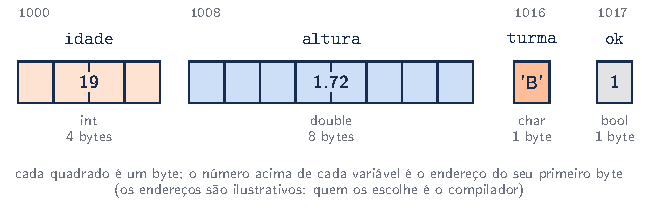
\includegraphics[width=0.9\linewidth,keepaspectratio]{imagens/capitulo-03_memoria.pdf}
\end{center}

Em C++, toda variável precisa ser \textbf{declarada} antes de ser usada, indicando o tipo e o nome. O ideal é já dar um valor inicial na declaração, o que se chama \textbf{inicializar}. Uma variável declarada sem valor contém o que estiver naquele pedaço da memória, um valor imprevisível conhecido como ``lixo''. O g++ avisa quando isso acontece: \texttt{\textquotesingle{}x\textquotesingle{} is used uninitialized}.

Quando um valor não deve mudar nunca, como o número $\pi$ ou a média mínima para aprovação, ele é declarado como \textbf{constante}, com a palavra \texttt{const}. Qualquer tentativa de alterá-lo vira um erro de compilação. Por convenção, nomes de constantes são escritos em maiúsculas.

\begin{codigo}
\begin{Verbatim}[breaklines=true, breaksymbolleft={}, fontsize=\footnotesize]
#include <iostream>
#include <string>
using namespace std;

int main() {
    int idade = 19;               // número inteiro
    double altura = 1.72;         // número real
    char turma = 'B';             // um caractere: aspas simples
    bool matriculado = true;      // verdadeiro ou falso
    string nome = "Ana Lima";     // texto: aspas duplas
    const double MEDIA_MINIMA = 6.0;   // constante

    idade = idade + 1;            // usa o antigo e o substitui
    cout << nome << ", " << idade << " anos, turma " << turma
         << endl;                  // Ana Lima, 20 anos, turma B
    cout << matriculado << endl;                // 1
    cout << boolalpha << matriculado << endl;   // true
    cout << "Média mínima: " << MEDIA_MINIMA << endl;   // 6
    return 0;
}
\end{Verbatim}
\end{codigo}

A linha \texttt{idade = idade + 1;} mostra como a atribuição funciona: primeiro o lado direito é calculado, usando o valor atual (19); depois o resultado (20) é guardado na variável da esquerda, substituindo o anterior. Para o \texttt{cout}, um \texttt{bool} verdadeiro aparece como 1; o \texttt{boolalpha} faz aparecer \texttt{true} e \texttt{false}.

\subsection{3.2 Tipos de dados}

O \textbf{tipo} de uma variável define três coisas: quais valores ela pode guardar, quanto espaço ocupa na memória e quais operações fazem sentido com ela. Os tipos básicos do C++ e seus equivalentes em Portugol são:

\begin{center}
\begin{tabular}{@{}p{0.15\linewidth}p{0.17\linewidth}p{0.36\linewidth}p{0.2\linewidth}@{}}
\toprule
\rowcolor{headergray}
\tblheader{C++} & \tblheader{Portugol} & \tblheader{Guarda} & \tblheader{Exemplos} \\
\midrule
\texttt{int} & \texttt{inteiro} & números inteiros & \texttt{19}, \texttt{-3} \\
\rowcolor{rowgray} \texttt{double} & \texttt{real} & números com casas decimais & \texttt{1.72}, \texttt{-0.5} \\
\texttt{char} & \texttt{caractere} & um único caractere & \texttt{\textquotesingle{}B\textquotesingle{}}, \texttt{\textquotesingle{}7\textquotesingle{}} \\
\rowcolor{rowgray} \texttt{bool} & \texttt{logico} & verdadeiro ou falso & \texttt{true}, \texttt{false} \\
\texttt{string} & \texttt{caractere} & um texto & \texttt{"Ana"} \\
\bottomrule
\end{tabular}
\end{center}

Repare que o Portugol usa \texttt{caractere} tanto para uma letra quanto para um texto inteiro, enquanto o C++ separa os dois: \texttt{char} guarda exatamente um caractere, entre aspas simples, e \texttt{string} guarda um texto, entre aspas duplas. \texttt{\textquotesingle{}A\textquotesingle{}} e \texttt{"A"} são coisas diferentes em C++.

Cada tipo tem um tamanho, e o tamanho limita os valores possíveis. O tamanho exato depende do compilador e do sistema, mas nos computadores atuais costuma ser o que o programa abaixo mostra. A função \texttt{sizeof} informa quantos bytes um tipo ocupa, e a biblioteca \texttt{<climits>} traz os limites de cada tipo inteiro.

\begin{codigo}
\begin{Verbatim}[breaklines=true, breaksymbolleft={}, fontsize=\footnotesize]
#include <iostream>
#include <climits>     // INT_MAX, LLONG_MAX
using namespace std;

int main() {
    cout << "int: " << sizeof(int) << " bytes, até "
         << INT_MAX << endl;       // 4 bytes, até 2147483647
    cout << "long long: " << sizeof(long long) << " bytes, até "
         << LLONG_MAX << endl;
    // 8 bytes, até 9223372036854775807
    cout << "double: " << sizeof(double) << endl;   // 8
    cout << "char: " << sizeof(char) << endl;       // 1
    cout << "bool: " << sizeof(bool) << endl;       // 1
    return 0;
}
\end{Verbatim}
\end{codigo}

Um \texttt{int} vai de cerca de $-2{,}1$ a $2{,}1$ bilhões. É suficiente para idades, quantidades e anos, mas não para a população mundial ou para valores em centavos de uma grande empresa: para esses, use \texttt{long long}. Quando uma conta passa do limite, acontece um \textbf{estouro} (\textit{overflow}), e o resultado fica errado sem nenhum aviso durante a execução.

O \texttt{double} guarda cerca de 15 dígitos significativos, o que é ótimo para medidas e cálculos científicos. Mas ele guarda os números em binário, e muitas frações que são exatas em decimal, como 0,1, não têm representação exata em binário. Por isso, \texttt{0.1 + 0.2} dá \texttt{0.30000000000000004}, e não exatamente \texttt{0.3}. Para a maioria das contas, essa diferença é irrelevante; ela só importa quando se compara valores reais com \texttt{==}, como você verá na Seção 3.5.

\subsection{3.3 Operadores aritméticos}

Os operadores aritméticos fazem as contas. Quase todos funcionam como na matemática, com duas atenções especiais: a divisão e o resto.

\begin{center}
\begin{tabular}{@{}p{0.2\linewidth}p{0.18\linewidth}p{0.18\linewidth}p{0.32\linewidth}@{}}
\toprule
\rowcolor{headergray}
\tblheader{Operação} & \tblheader{C++} & \tblheader{Portugol} & \tblheader{Exemplo em C++} \\
\midrule
soma & \texttt{+} & \texttt{+} & \texttt{17 + 5} vale 22 \\
\rowcolor{rowgray} subtração & \texttt{-} & \texttt{-} & \texttt{17 - 5} vale 12 \\
multiplicação & \texttt{*} & \texttt{*} & \texttt{17 * 5} vale 85 \\
\rowcolor{rowgray} divisão & \texttt{/} & \texttt{/} ou \texttt{div} & \texttt{17 / 5} vale 3 \\
resto & \texttt{\%} & \texttt{mod} ou \texttt{\%} & \texttt{17 \% 5} vale 2 \\
\rowcolor{rowgray} potência & \texttt{pow(a, b)} & \texttt{\textasciicircum} & \texttt{pow(2, 10)} vale 1024 \\
\bottomrule
\end{tabular}
\end{center}

Em C++, o operador \texttt{/} faz \textbf{divisão inteira} quando os dois lados são inteiros: \texttt{17 / 5} vale 3, e a parte decimal é descartada (não há arredondamento: \texttt{19 / 5} também vale 3). Se pelo menos um dos lados for real, a divisão é real: \texttt{17.0 / 5} vale 3.4. No Portugol do VisuAlg, \texttt{/} é sempre a divisão real, e a inteira se escreve \texttt{div}.

O operador \texttt{\%} dá o \textbf{resto} da divisão inteira, e é muito mais útil do que parece: \texttt{n \% 2} é 0 quando \texttt{n} é par; \texttt{n \% 10} é o último dígito de \texttt{n}; \texttt{n \% 7} diz em que dia da semana cai o dia \texttt{n} de uma contagem. Ele só funciona com inteiros.

Quando uma expressão tem vários operadores, a \textbf{precedência} decide a ordem: multiplicação, divisão e resto vêm antes de soma e subtração, e operadores do mesmo nível são calculados da esquerda para a direita. Parênteses mudam a ordem, e vale a pena usá-los sempre que deixarem a intenção mais clara.

\begin{codigo}
\begin{Verbatim}[breaklines=true, breaksymbolleft={}, fontsize=\footnotesize]
#include <iostream>
using namespace std;

int main() {
    int a = 17, b = 5;
    cout << a + b << " " << a - b << " " << a * b << endl;
    // 22 12 85
    cout << a / b << endl;              // 3: divisão inteira
    cout << a % b << endl;              // 2: resto
    cout << 17.0 / 5 << endl;           // 3.4
    cout << static_cast<double>(a) / b << endl;   // 3.4
    cout << 2 + 3 * 4 << " " << (2 + 3) * 4 << endl;  // 14 20
    cout << 1234 % 10 << " " << 1234 / 10 << endl;    // 4 123

    int pontos = 10;
    pontos += 5;       // o mesmo que pontos = pontos + 5: 15
    pontos++;          // soma 1: 16
    pontos *= 2;       // o mesmo que pontos = pontos * 2: 32
    pontos--;          // subtrai 1: 31
    cout << pontos << endl;             // 31
    return 0;
}
\end{Verbatim}
\end{codigo}

O \texttt{static\_cast<double>(a)} converte o valor de \texttt{a} para \texttt{double} só naquela conta, sem mudar a variável; com isso, a divisão passa a ser real. Os operadores \texttt{+=}, \texttt{-=}, \texttt{*=} e \texttt{/=} são atalhos para alterar uma variável usando o próprio valor dela, e \texttt{++} e \texttt{--} somam e subtraem 1. Eles aparecem o tempo todo nas repetições do Capítulo 5.

\subsection{3.4 Conversões de tipo}

Quando valores de tipos diferentes se encontram em uma conta ou atribuição, o C++ converte um deles. As conversões que não perdem informação, como de \texttt{int} para \texttt{double}, são feitas sem problema. As que perdem informação exigem cuidado:

\begin{codigo}
\begin{Verbatim}[breaklines=true, breaksymbolleft={}, fontsize=\footnotesize]
#include <iostream>
#include <cmath>       // round
using namespace std;

int main() {
    double preco = 9.99;
    int reais = static_cast<int>(preco);   // 9: corta os decimais
    cout << reais << " " << round(preco) << endl;   // 9 10

    int quantidade = 7;
    double metade = quantidade / 2.0;      // 3.5
    cout << metade << endl;

    char letra = 'A';
    cout << static_cast<int>(letra) << endl;        // 65
    cout << static_cast<char>(letra + 2) << endl;   // C
    return 0;
}
\end{Verbatim}
\end{codigo}

Converter um \texttt{double} para \texttt{int} \textbf{corta} a parte decimal, sem arredondar: 9,99 vira 9. Para arredondar, use \texttt{round}, da biblioteca \texttt{<cmath>}. A conversão entre \texttt{char} e \texttt{int} mostra que, para o computador, cada caractere é um número: o código do \texttt{\textquotesingle{}A\textquotesingle{}} na tabela ASCII é 65, o do \texttt{\textquotesingle{}B\textquotesingle{}} é 66, e assim por diante. Por isso \texttt{\textquotesingle{}A\textquotesingle{} + 2} dá 67, o código do \texttt{\textquotesingle{}C\textquotesingle{}}.

\subsection{3.5 Operadores relacionais}

Os operadores relacionais comparam dois valores e dão como resultado um \texttt{bool}: \texttt{true} ou \texttt{false}. São eles que formam as condições das decisões e repetições dos próximos capítulos.

\begin{center}
\begin{tabular}{@{}p{0.3\linewidth}p{0.18\linewidth}p{0.18\linewidth}p{0.2\linewidth}@{}}
\toprule
\rowcolor{headergray}
\tblheader{Pergunta} & \tblheader{C++} & \tblheader{Portugol} & \tblheader{Com x = 7} \\
\midrule
igual a & \texttt{==} & \texttt{=} & \texttt{x == 7} é \texttt{true} \\
\rowcolor{rowgray} diferente de & \texttt{!=} & \texttt{<>} & \texttt{x != 7} é \texttt{false} \\
maior que & \texttt{>} & \texttt{>} & \texttt{x > 7} é \texttt{false} \\
\rowcolor{rowgray} menor que & \texttt{<} & \texttt{<} & \texttt{x < 10} é \texttt{true} \\
maior ou igual a & \texttt{>=} & \texttt{>=} & \texttt{x >= 7} é \texttt{true} \\
\rowcolor{rowgray} menor ou igual a & \texttt{<=} & \texttt{<=} & \texttt{x <= 6} é \texttt{false} \\
\bottomrule
\end{tabular}
\end{center}

Atenção à igualdade: em C++, \texttt{=} é \textbf{atribuição} e \texttt{==} é \textbf{comparação}. No Portugol é o contrário, porque a atribuição é a seta \texttt{<-}, e \texttt{=} compara. Escrever \texttt{x = 7} onde se queria \texttt{x == 7} é um dos erros mais comuns em C++, e o Capítulo 4 mostra por que ele é tão traiçoeiro.

Também por causa da representação em binário, não compare valores \texttt{double} com \texttt{==}: \texttt{0.1 + 0.2 == 0.3} dá \texttt{false}. Em vez disso, verifique se a diferença entre eles é muito pequena, por exemplo menor que \texttt{0.000001}.

\subsection{3.6 Operadores lógicos}

Os operadores lógicos combinam condições, exatamente como os conectivos E, OU e NÃO do Capítulo 1, com a mesma tabela-verdade:

\begin{center}
\begin{tabular}{@{}p{0.2\linewidth}p{0.16\linewidth}p{0.18\linewidth}p{0.32\linewidth}@{}}
\toprule
\rowcolor{headergray}
\tblheader{Conectivo} & \tblheader{C++} & \tblheader{Portugol} & \tblheader{Verdadeiro quando} \\
\midrule
E & \texttt{\&\&} & \texttt{e} & as duas condições são verdadeiras \\
\rowcolor{rowgray} OU & \texttt{||} & \texttt{ou} & pelo menos uma é verdadeira \\
NÃO & \texttt{!} & \texttt{nao} & a condição é falsa \\
\bottomrule
\end{tabular}
\end{center}

\begin{codigo}
\begin{Verbatim}[breaklines=true, breaksymbolleft={}, fontsize=\footnotesize]
#include <iostream>
using namespace std;

int main() {
    double nota = 7.5;
    int frequencia = 80;              // em %
    int idade = 17;
    bool estudante = true;

    bool aprovado = nota >= 6 && frequencia >= 75;
    bool meiaEntrada = estudante || idade >= 60;
    bool menor = !(idade >= 18);
    bool notaValida = nota >= 0 && nota <= 10;

    cout << boolalpha;
    cout << aprovado << " " << meiaEntrada << endl;   // true true
    cout << menor << " " << notaValida << endl;       // true true
    cout << (0.1 + 0.2 == 0.3) << endl;               // false
    return 0;
}
\end{Verbatim}
\end{codigo}

Repare em \texttt{notaValida}: para dizer ``a nota está entre 0 e 10'', é preciso escrever as duas comparações ligadas por \texttt{\&\&}. A forma matemática \texttt{0 <= nota <= 10} compila, mas não faz o que parece: o C++ calcula \texttt{0 <= nota}, que dá \texttt{true} ou \texttt{false} (1 ou 0), e depois compara esse 1 ou 0 com 10, o que é sempre verdadeiro. O g++ avisa: \texttt{comparisons like \textquotesingle{}X<=Y<=Z\textquotesingle{} do not have their mathematical meaning}.

Os operadores \texttt{\&\&} e \texttt{||} também fazem \textbf{avaliação em curto-circuito}: se a resposta já está decidida pelo lado esquerdo, o lado direito nem é calculado. Em \texttt{pessoas > 0 \&\& total / pessoas > 50}, se \texttt{pessoas} for 0, a divisão por zero nunca acontece, porque \texttt{pessoas > 0} já é falso e o \texttt{\&\&} só pode dar falso.

\subsection{3.7 Precedência geral}

Com operadores de tipos diferentes na mesma expressão, a ordem de cálculo segue esta tabela, do primeiro para o último:

\begin{center}
\begin{tabular}{@{}p{0.1\linewidth}p{0.36\linewidth}p{0.42\linewidth}@{}}
\toprule
\rowcolor{headergray}
\tblheader{Ordem} & \tblheader{Operadores} & \tblheader{Tipo} \\
\midrule
1 & \texttt{( )} & parênteses \\
\rowcolor{rowgray} 2 & \texttt{!}, \texttt{-} (negativo), \texttt{++}, \texttt{--} & unários \\
3 & \texttt{*}, \texttt{/}, \texttt{\%} & multiplicação, divisão e resto \\
\rowcolor{rowgray} 4 & \texttt{+}, \texttt{-} & soma e subtração \\
5 & \texttt{<}, \texttt{<=}, \texttt{>}, \texttt{>=} & relacionais \\
\rowcolor{rowgray} 6 & \texttt{==}, \texttt{!=} & igualdade \\
7 & \texttt{\&\&} & e lógico \\
\rowcolor{rowgray} 8 & \texttt{||} & ou lógico \\
9 & \texttt{=}, \texttt{+=}, \texttt{-=}, ... & atribuição \\
\bottomrule
\end{tabular}
\end{center}

A figura mostra a avaliação de uma expressão que mistura quase todos eles:

\begin{center}
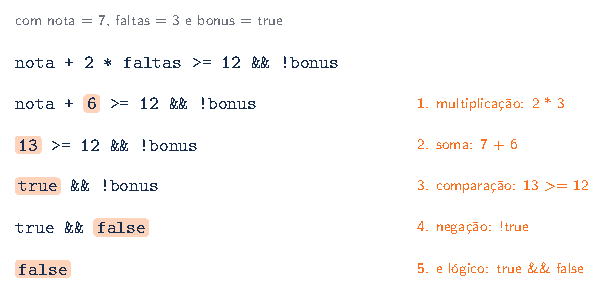
\includegraphics[width=0.85\linewidth,keepaspectratio]{imagens/capitulo-03_avaliacao.pdf}
\end{center}

Note que \texttt{\&\&} vem antes de \texttt{||}: \texttt{a || b \&\& c} significa \texttt{a || (b \&\& c)}. Ninguém precisa decorar a tabela inteira: na dúvida, use parênteses. Eles nunca atrapalham e deixam claro para quem lê o que se pretendia.

\subsection{3.8 Funções matemáticas}

A biblioteca \texttt{<cmath>} traz as funções matemáticas mais usadas:

\begin{center}
\begin{tabular}{@{}p{0.26\linewidth}p{0.4\linewidth}p{0.24\linewidth}@{}}
\toprule
\rowcolor{headergray}
\tblheader{Função} & \tblheader{Calcula} & \tblheader{Exemplo} \\
\midrule
\texttt{sqrt(x)} & raiz quadrada & \texttt{sqrt(16)} é 4 \\
\rowcolor{rowgray} \texttt{pow(x, y)} & $x$ elevado a $y$ & \texttt{pow(2, 10)} é 1024 \\
\texttt{abs(x)} & valor absoluto & \texttt{abs(-7)} é 7 \\
\rowcolor{rowgray} \texttt{round(x)} & arredonda para o inteiro mais próximo & \texttt{round(2.5)} é 3 \\
\texttt{floor(x)} & arredonda para baixo & \texttt{floor(2.7)} é 2 \\
\rowcolor{rowgray} \texttt{ceil(x)} & arredonda para cima & \texttt{ceil(2.1)} é 3 \\
\bottomrule
\end{tabular}
\end{center}

O \texttt{ceil} resolve com facilidade problemas do tipo ``quantos ônibus de 40 lugares são necessários para 130 alunos?'': \texttt{ceil(130 / 40.0)} dá 4. Com a divisão inteira \texttt{130 / 40}, o resultado seria 3, e 10 alunos ficariam para trás.

\subsection{3.9 Um programa completo}

Um sistema de vídeos registra a duração em segundos, mas precisa mostrá-la em horas, minutos e segundos. A divisão inteira e o resto resolvem o problema: cada hora tem 3600 segundos, então \texttt{total / 3600} dá as horas completas; o que sobra, \texttt{total \% 3600}, dividido por 60, dá os minutos; e \texttt{total \% 60} dá os segundos restantes.

\begin{codigo}
\begin{Verbatim}[breaklines=true, breaksymbolleft={}, fontsize=\footnotesize]
algoritmo "ConverterSegundos"
var
   total, horas, minutos, segundos: inteiro
inicio
   escreva("Duração em segundos: ")
   leia(total)
   horas <- total div 3600
   minutos <- (total mod 3600) div 60
   segundos <- total mod 60
   escreval(horas, "h ", minutos, "min ", segundos, "s")
fimalgoritmo
\end{Verbatim}
\end{codigo}

\begin{codigo}
\begin{Verbatim}[breaklines=true, breaksymbolleft={}, fontsize=\footnotesize]
#include <iostream>
using namespace std;

int main() {
    int total;
    cout << "Duração em segundos: ";
    cin >> total;
    int horas = total / 3600;
    int minutos = (total % 3600) / 60;
    int segundos = total % 60;
    cout << horas << "h " << minutos << "min " << segundos << "s"
         << endl;
    return 0;
}
// Exemplo de execução:
// Duração em segundos: 3725
// 1h 2min 5s
\end{Verbatim}
\end{codigo}

Um teste de mesa confirma: $3725 / 3600 = 1$ hora; $3725 \bmod 3600 = 125$, e $125 / 60 = 2$ minutos; $3725 \bmod 60 = 5$ segundos. Conferindo: $3600 + 2 \times 60 + 5 = 3725$.

\subsection{Erros Comuns}

\begin{itemize}
  \item \textbf{Usar uma variável sem inicializá-la.} Ela contém lixo, e o resultado muda a cada execução. Dê sempre um valor inicial.
  \item \textbf{Dividir inteiros esperando casas decimais.} \texttt{7 / 2} vale 3. Use \texttt{7.0 / 2} ou \texttt{static\_cast<double>}.
  \item \textbf{Confundir \texttt{=} com \texttt{==}.} \texttt{=} atribui; \texttt{==} compara.
  \item \textbf{Escrever \texttt{0 <= x <= 10}.} Compila, mas é sempre verdadeiro. Use \texttt{x >= 0 \&\& x <= 10}.
  \item \textbf{Comparar \texttt{double} com \texttt{==}.} \texttt{0.1 + 0.2 == 0.3} é falso. Compare a diferença com uma tolerância pequena.
  \item \textbf{Confundir \texttt{\textquotesingle{}A\textquotesingle{}} com \texttt{"A"}.} Aspas simples são um \texttt{char}; aspas duplas, um texto.
  \item \textbf{Esperar que a conversão para \texttt{int} arredonde.} Ela corta: 9,99 vira 9. Use \texttt{round}.
  \item \textbf{Estourar o \texttt{int}.} Contas que passam de 2,1 bilhões dão resultados errados. Use \texttt{long long} para números grandes.
  \item \textbf{Usar \texttt{\%} com números reais.} O resto só existe para inteiros; com \texttt{double}, é erro de compilação.
\end{itemize}
